% !TeX root = ../defense.tex

\section{Results, Conclusion and Further Work}
\frame{\sectionpage}

\begin{frame}{Data Distribution}
    The data obtained by executing all the orderings for the query plan on Linear road data, resulted in the following frequencies for optimal orderings.
    \begin{figure}
        \centering
        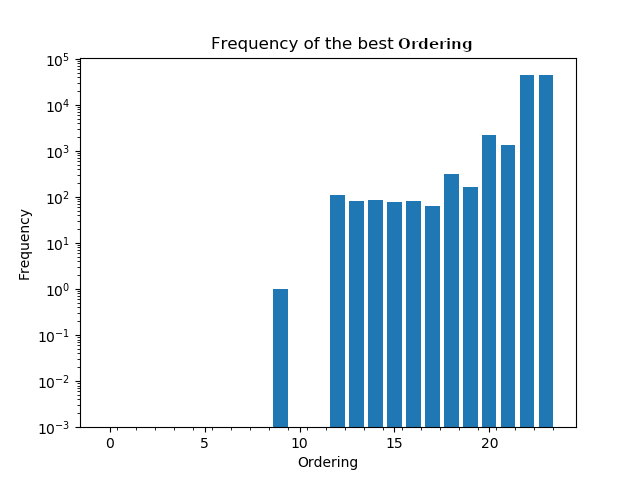
\includegraphics[scale=0.375]{totalb1.png}\\
        \caption{This figure shows the frequency distribution of the number of cases where each move is optimal}
        \label{fig:totalb1}
    \end{figure}
\end{frame}


\begin{frame}{Data Distribution}
    While training and testing the DQN model, we divided the total data into a $70:30$ for training and testing purposes respectively.
    \begin{figure}
        \centering
        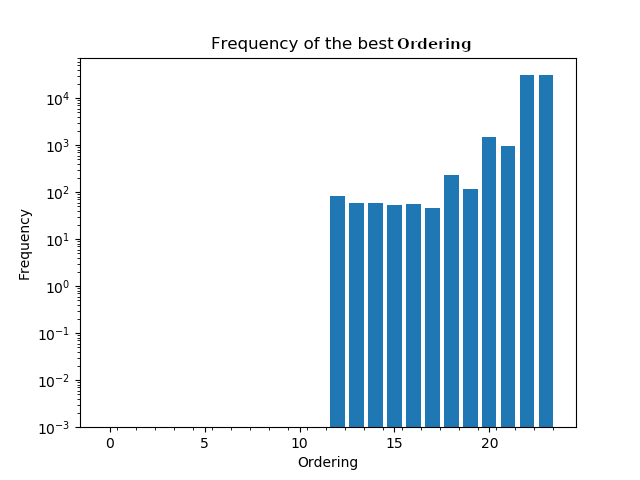
\includegraphics[scale=0.375]{trainingb1.png}\\
        \caption{This figure shows the frequency distribution of cases where each move is optimal in the training dataset}
        \label{fig:trainingb1}
    \end{figure}
\end{frame}

\begin{frame}{Data Distribution}
    While training and testing the DQN model, we divided the total data into a $70:30$ for training and testing purposes respectively.
    \begin{figure}
        \centering
        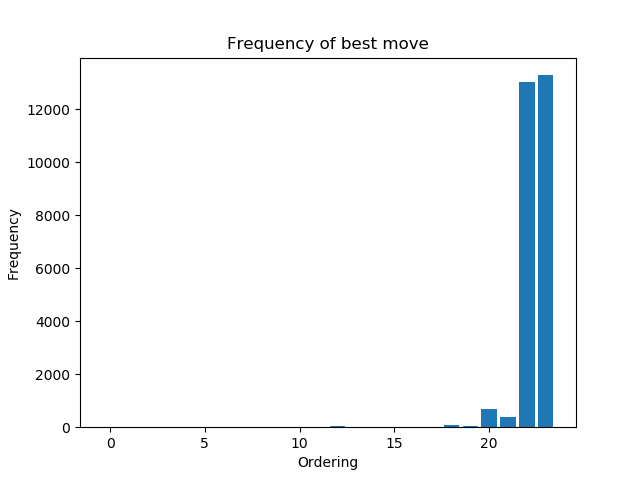
\includegraphics[scale=0.375]{testingb1.png}\\
        \caption{This figure shows the frequency distribution of cases where each move is optimal in the testing dataset}
        \label{fig:testingb1}
    \end{figure}
\end{frame}


\begin{frame}{Confusion Matrix}
    The predictions on trained model lead to the following confusion matrix.
    \begin{figure}
        \centering
        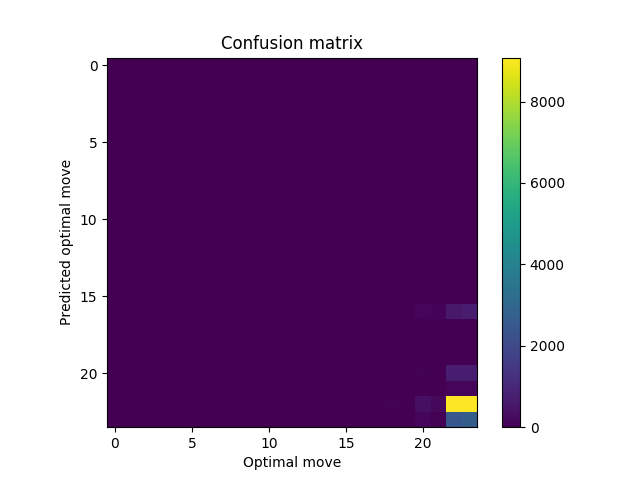
\includegraphics[scale=0.5]{cm1.png}\\
        \caption{DQN Run 1 confusion matrix}
        \label{fig:dqn_r1_1}
    \end{figure}
\end{frame}

\begin{frame}{Confusion Matrix}
    The predictions on trained model lead to the following confusion matrix.
    \begin{figure}
        \centering
        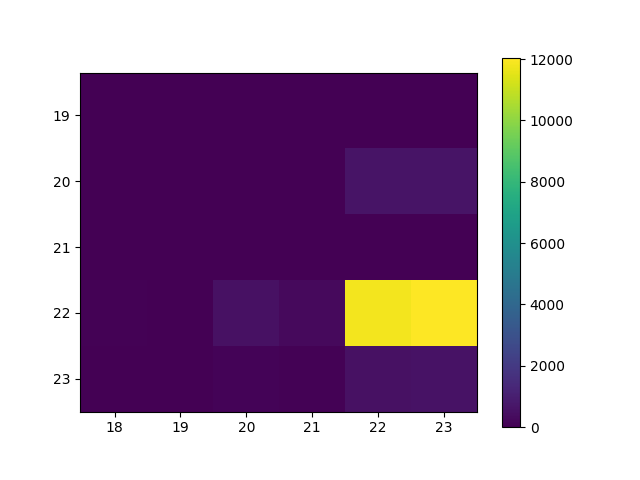
\includegraphics[scale=0.3]{cm3.png}\\
        \caption{DQN Run 2 confusion matrix}
        \label{fig:dqn_r2_1}
    \end{figure}
\end{frame}

\begin{frame}{Predictions}
    Some of the cases we were able to predict the correct answers.
    \begin{figure}
        \centering
        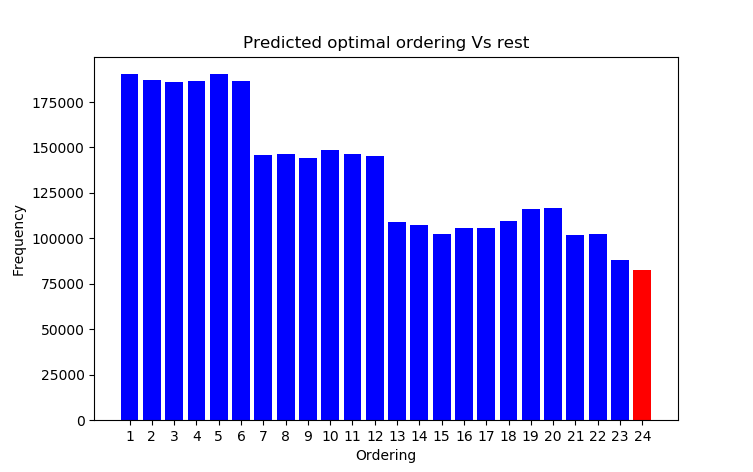
\includegraphics[scale=0.4]{operations1.png}\\
        \caption{The figure shows the log$_{10}$(number of operations) required to execute the query depending on the ordering of the selection operators chosen. The predicted optimal ordering is shown in red.}
        \label{fig:operations1}
    \end{figure}
\end{frame}

\begin{frame}{Predictions}
    Some of the cases we were able to predict the correct answers.
    \begin{figure}
        \centering
        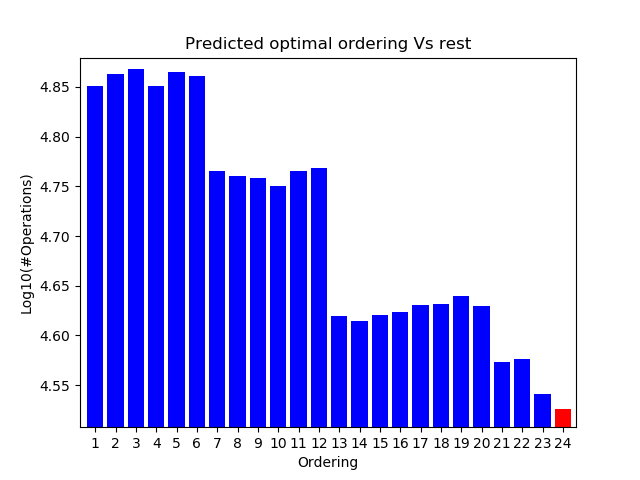
\includegraphics[scale=0.4]{operations2.png}\\
        \caption{The figure shows the log$_{10}$(number of operations) required to execute the query depending on the ordering of the selection operators chosen. The predicted optimal ordering is shown in red.}
        \label{fig:operations2}
    \end{figure}
\end{frame}

\begin{frame}{Overall Performance}
    The model predicted optimal move correctly for $12978$ data points, out of $27681$, i.e. $47\%$.\\
\end{frame}

\begin{frame}{Overall Performance}
    \begin{enumerate}[<+->]
        \item The sum of operations required by the optimal ordering $890640075.0$
        \item The sum of operations required by the predicted ordering $900269878.0$
        \item The sum of operations required by the optimal ordering $2310227856.0$
    \end{enumerate}
\end{frame}

\begin{frame}
    Our model resulted in requiring $39\%$ of operations as the query execution would have required if it executed the worst ordering every time.\\
    Our model resulted in requiring $102\%$ of operations as the query execution would have required if it executed the optimal ordering every time.\\
\end{frame}

\begin{frame}{Further Work}
    \begin{itemize}[<+->]
        \item The neural network is unable to achieve low loss for the test data, this perhaps speak the lack of features extracted during the querying time.
        \item The data sample we have is highly biased, leading to rather baised DQNs.
        \item The entire method needs to be parallelized and set up on a scalable infrastructure to see the actual effects of DQN.
        \item The DQN used is simulating a single move game rather than a multi move game.
        \item Not looked at how DQNs can be trained online.
    \end{itemize}
\end{frame}

\begin{frame}{}
    Questions?
\end{frame}

